\documentclass[14pt]{beamer}
\usepackage[italian]{babel}
\usepackage[utf8]{inputenc}
\usepackage{graphicx}
\mode<presentation>
\usetheme{Madrid}

\title[Parallelismo e Haskell]{Parallelismo e Haskell} % The short title appears at the bottom of every slide, the full title is only on the title page

\author{Jacopo Francesco Zemella} % Your name
\institute[Unimi] % Your institution as it will appear on the bottom of every slide, may be shorthand to save space
{
Università degli studi di Milano \\[2ex] % Your institution for the title page
\medskip
\textit{jacopofrancesco.zemella@studenti.unimi.it} % Your email address
}


\begin{document}

\begin{frame}
\titlepage
\end{frame}


\section{Algoritmi Sequenziali} 


\begin{frame}
\frametitle{Algoritmi Sequenziali}
\textbf{Algoritmo:} Sequenza finita di istruzioni interpretabili da un determinato agente, finalizzate a risolvere un problema\\[2ex]
\textbf{Calcolo Sequenziale}: Le istruzioni vengono eseguite in \textit{sequenza}, una dopo l'altra da una singola CPU: ad ogni istante di tempo è in esecuzione una e una sola operazione
\end{frame}


\section{Algoritmi Paralleli} 
\frame
{
	\frametitle{Algoritmi Paralleli}
	\textbf{Calcolo Parallelo}: Le istruzioni vengono eseguite su più processori contemporaneamente\\[2ex]
  \begin{figure}
    \centering
    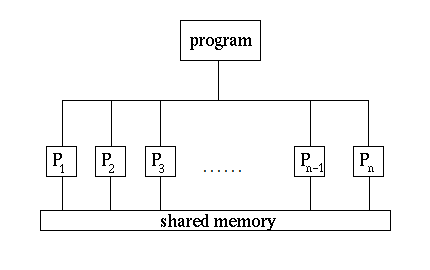
\includegraphics[width=8 cm]{./pram}
  \end{figure}

}


\begin{frame}
\frametitle{Legge di Amdahl - Limiti della Parallelizzazione}
\textit{"Il miglioramento che si può ottenere su una certa parte del sistema è limitato dalla frazione di tempo in cui tale attività ha luogo"}\\[2ex]
Analogamente il guadagno prestazionale ottenuto dal parallelismo è limitato dalla sua componente sequenziale intrinseca.
\end{frame}


\section{Haskell}
\begin{frame}
\frametitle{Haskell: Caratteristiche} 
\begin{itemize}
\item Linguaggio funzionale
\item Tipizzazione statica
\item Lazy evaluation
\item Trasparenza referenziale
 \item Particolarmente indicato per la parallelizzazione
  \begin{itemize}
  \item \textbf{GpH}: Glasgow parallel Haskell
  \end{itemize}

\end{itemize}
\end{frame}


\begin{frame}
\frametitle{Le sfide della Programmazione Parallela}
Implementare un programma parallelo richiede di specificare:
\begin{itemize}
\item \textbf{computazione}: creare un algoritmo  efficiente e corretto
\item \textbf{coordinamento}: gestire l'esecuzione per ottenere un "buon" livello di parallelismo
\end{itemize}
In Parallel Haskell \textbf{computazione} e \textbf{coordinamento} sono strettamente separate.
\end{frame}

\begin{frame}
\frametitle{Aspetti di coordinazione}
Coordinare l'andamento parallelo dell'esecuzione prevede, tra le altre cose:
\begin{itemize}
\item partizionamento: quali threads creare e la quantità di lavoro che devono svolgere
\item sincronizzazione tra i threads
\item load-store management
\item comunicazione 
\end{itemize}
\end{frame}


\begin{frame}
\frametitle{Glasgow Parallel Haskell}
\begin{itemize}
\item GpH è un'estensione \textbf{conservativa} di Haskell che permette di
  realizzare parallelismo \textbf{semi-esplicito} basato su threads.

\item Solo alcuni aspetti chiave devono essere specificati dal programmatore 
\item 
  Fornisce una sola primitiva per creare un thread, ma una volta creati essi sono gestiti autonomamente da un sofisticato sistema runtime.\\ [2ex]
\end{itemize}
% Inoltre le Strategies uniscono le primitive per la creazione dei thread con funzioni higher-order, consentendo astrazioni di coordinazione di alto livello.
\end{frame}

\begin{frame}
\frametitle{Parallelismo in GpH}
GpH mette a disposizione varie metodologie di programmazione parallela:
\begin{itemize}
\item Parallelismo semi-esplicito: funzioni \textit{par} e \textit{pseq}
\item Monade Eval e Strategie di valutazione
\item Dataflow Parallelism: Monade Par
\end{itemize}
Nella tesi abbiamo utilizzato le prime due, e in questa presentazione presentiamo solo la prima.
\end{frame}

\begin{frame}[fragile]
\frametitle{par e pseq}
Le due funzioni hanno la seguente segnature: 
\begin{verbatim}
par   :: a -> b -> b
pseq  :: a -> b -> b
\end{verbatim}
\begin{itemize}
\item La funzione
\textit{par} segnala il   primo argomento come un thread
"parallelizzabile" (spark), ovvero che la sua valutazione in parallelo
potrebbe essere conveniente
\item Tuttavia, poiché la \emph{lazy evaluation} di Haskell non impone
  un ordine di valutazione \textbf{stretto}, abbiamo bisogno anche di
  \textit{pseq}, che assicura che il primo argomento venga valutato
  prima del secondo.
\end{itemize}

\end{frame}


\begin{frame}[fragile]
\frametitle{Un esempio in Parallel Haskell \hfill 1/2}
Fattoriale \emph{divide et impera}: Caso Sequenziale
\small 
\begin{verbatim}
fact n = fact' 1 n

fact' :: Integer -> Integer -> Integer
fact' m n
  | m == n    = m
  | otherwise = left * right
      where 
          mid   = (m + n) `div` 2
          left  = fact' m mid
          right = fact' (mid+1) n
\end{verbatim}
\end{frame}

\begin{frame}[fragile]
\frametitle{Un esempio in Parallel Haskell \hfill 2/2}
Fattoriale: Caso Parallelo
\small 
\begin{verbatim}
pfact n = pfact' 1 n

pfact' :: Integer -> Integer -> Integer
pfact' m n
  | m == n    = m
  | otherwise = left `par` right `pseq` (left * right)
      where 
          mid   = (m + n) `div` 2
          left  = pfact' m mid
          right = pfact' (mid+1) n
\end{verbatim}
\end{frame}

\begin{frame}
\frametitle{Coordinamento\hfill 1/2}
Sfruttando le due funzioni otteniamo il parallelismo desiderato.\\[2ex]
\texttt{left `par` right `pseq` (left * right)}
\begin{figure}
    \centering
    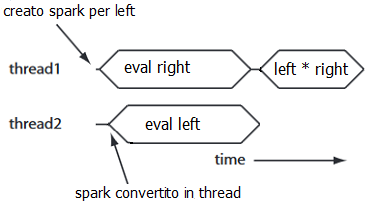
\includegraphics[width=6 cm]{./desired_par}
  \end{figure}
\end{frame}

\begin{frame}[fragile]
\frametitle{Coordinamento\hfill 2/2}
% Come abbiamo detto specificare le componenti parallele del programma non è sufficiente: dobbiamo controllare l'ordine della valutazione.
Se avessimo scritto la funzione come segue:
\begin{verbatim}
  | otherwise = left `par` (left * right)
\end{verbatim}
la somma avrebbe potuto valutare \textit{left} sul core principale, prima che qualsiasi altro avesse la possibilità di calcolarlo.
\begin{figure}
    \centering
    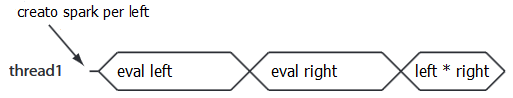
\includegraphics[width=8 cm]{./not_desired_par}
  \end{figure}


La \textit{`pseq`} assicura che \textit{left} e \textit{right} siano calcolate in parallelo prima di moltiplicarle.
\end{frame}

% \begin{frame}
% La mancata coordinazione sfocia in eventi di questo tipo.\\[2ex]
% \texttt{left `par` (left * right)}
% \begin{figure}
%     \centering
%     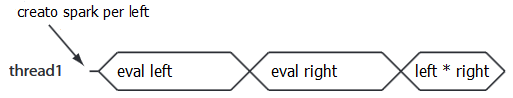
\includegraphics[width=8 cm]{./not_desired_par}
%   \end{figure}
% \end{frame}

\begin{frame}
\frametitle{Problemi Implementati e Risolti nel Tirocinio}
\begin{itemize}
\item Sorting: 
		\begin{itemize}
			\item quicksort
			\item mergesort
		\end{itemize}
\item Algebra Lineare:
		\begin{itemize}
			\item Somma, prodotto, potenza di Matrici
			\item Calcolo del determinante
			\item Inversione di una matrice
		\end{itemize}
\item Grafi:
		\begin{itemize}
			\item Connettività
		\end{itemize}
\end{itemize}
\end{frame}

\begin{frame}
\frametitle{Conclusioni e Sviluppi Futuri}
Haskell offre un ampio numero di implementazioni per la programmazione parallela mediante una semantica di comodo utilizzo.\\[2pt]
Possibili sviluppi:
\begin{itemize}
\item Valutazione empirica del tempo di esecuzione degli esempi implementati.
\item Confronto delle varie metodologie di programmazione.
\item Analisi delle altre tecniche di parallelizzazione non affrontate
  nel tirocinio.
\end{itemize}
\end{frame}

\begin{frame}
\Huge{\centerline{Grazie per l'attenzione!}}
\end{frame}

\end{document}